\documentclass[11pt]{article}

\newcommand{\StudentName}{Gabriel Molina Bulgarelli}
\newcommand{\StudentID}{C14826}
\newcommand{\CourseName}{CI-0146 Compilers}
\newcommand{\InstructorName}{Dr. Francisco J. Torres-Rojas}
\newcommand{\AcademicTerm}{Second Semester 2026}
\newcommand{\AssignmentTitle}{GCC Constant Folding and Constant Propagation}
\newcommand{\SubmissionDate}{September 3, 2026}


\usepackage[utf8]{inputenc}
\usepackage[T1]{fontenc}
\usepackage[english]{babel}
\usepackage{lmodern}
\usepackage{microtype}
\usepackage[margin=1in]{geometry}
\usepackage{graphicx}
\usepackage{booktabs}
\usepackage{array}
\usepackage{listings}
\usepackage{xcolor}
\usepackage{caption}
\usepackage{float}
\usepackage{fancyhdr}
\usepackage{hyperref}

\definecolor{navy}{HTML}{17365D}
\definecolor{blue}{HTML}{245B8A}
\definecolor{codeback}{HTML}{F4F6F8}
\definecolor{codeframe}{HTML}{CAD3DC}
\definecolor{commentgreen}{HTML}{3F6B4F}

\hypersetup{
  colorlinks=true,
  linkcolor=navy,
  urlcolor=blue,
  pdftitle={\AssignmentTitle},
  pdfauthor={\StudentName}
}

\lstdefinestyle{code}{
  basicstyle=\ttfamily\small,
  backgroundcolor=\color{codeback},
  frame=single,
  rulecolor=\color{codeframe},
  numbers=left,
  numberstyle=\scriptsize\color{gray},
  numbersep=8pt,
  showstringspaces=false,
  columns=fullflexible,
  keepspaces=true,
  breaklines=true,
  commentstyle=\color{commentgreen},
  keywordstyle=\color{navy}\bfseries,
  aboveskip=0.8em,
  belowskip=0.8em
}
\lstset{style=code}

\pagestyle{fancy}
\fancyhf{}
\lhead{\CourseName}
\rhead{Exercise 1.4}
\cfoot{\thepage}
\setlength{\headheight}{14pt}

\newcommand{\code}[1]{\texttt{#1}}
\newcommand{\answerline}[1]{\par\noindent\textcolor{navy}{\textbf{Answer:}} #1\par}

\begin{document}
\pagenumbering{gobble}

\begin{titlepage}
  \centering
  \vspace*{1.2in}
  {\Large \CourseName\par}
  \vspace{0.25in}
  {\large \AcademicTerm\par}
  \vspace{0.85in}
  {\color{navy}\rule{\textwidth}{1.2pt}\par}
  \vspace{0.28in}
  {\Huge\bfseries \AssignmentTitle\par}
  \vspace{0.18in}
  {\Large Exercise 1.4: Experimental Study with GCC\par}
  \vspace{0.28in}
  {\color{navy}\rule{\textwidth}{1.2pt}\par}
  \vfill
  \begin{tabular}{>{\bfseries}r l}
    Student: & \StudentName \\
    Student ID: & \StudentID \\
    Instructor: & \InstructorName \\
    Due date: & \SubmissionDate \\
  \end{tabular}
  \vfill
\end{titlepage}

\pagenumbering{roman}
\tableofcontents
\clearpage
\pagenumbering{arabic}

\section{Assignment Statement}

\subsection{Instructor instructions}

\begin{quote}
Solve the exercise shown at the end of this message using GCC on Linux as the
case study. Capture screenshots of the GCC executions required to construct
your answers.

Prepare a LaTeX document containing all of your work, using any style you
prefer, but it must be of high quality. Submit a printed copy at the beginning
of class on Thursday, September 3. Also send the LaTeX source and all files
required to compile it to the specified email address before the corresponding
class.

If the work does not comply with these specifications, or if it is submitted
without the problem statements, without names, or with incomplete information,
the grade will immediately be zero.
\end{quote}

\subsection{Exercise 1.4}

This question assumes that you have a compiler that has an option to produce
assembly language output.

\medskip
\noindent\textbf{a.} Determine if your compiler performs constant folding
optimizations.

\medskip
\noindent\textbf{b.} A related but more advanced optimization is that of
constant propagation: a variable that currently has a constant value is
replaced by that value in expressions. For example, the code (in C syntax)

\begin{lstlisting}[language=C,numbers=none]
x = 4;
y = x + 2;
\end{lstlisting}

would, using constant propagation (and constant folding), be replaced by the
code

\begin{lstlisting}[language=C,numbers=none]
x = 4;
y = 6;
\end{lstlisting}

Determine if your compiler performs constant propagation.

\medskip
\noindent\textbf{c.} Give as many reasons as you can why constant propagation
is more difficult than constant folding.

\medskip
\noindent\textbf{d.} A situation related to constant propagation and constant
folding is the use of named constants in a program. Using a named constant
\code{x} instead of a variable, we can translate the above example as the
following C code:

\begin{lstlisting}[language=C,numbers=none]
const int x = 4;
...
y = x + 2;
...
\end{lstlisting}

Determine if your compiler performs propagation/folding under these
circumstances.

How is this different from part (b)?

\clearpage
\section{Environment and Methodology}

All measurements in this report were taken directly on the system summarized
in Table~\ref{tab:environment}. The screenshots are retained records of those
executions; the typeset listings are used for close technical inspection.

\begin{table}[H]
  \centering
  \caption{Recorded compiler and operating-system environment.}
  \label{tab:environment}
  \begin{tabular}{@{}>{\bfseries}p{0.28\textwidth}p{0.64\textwidth}@{}}
    \toprule
    Component & Recorded value \\
    \midrule
    Compiler & GCC 16.1.1 20260515 (Red Hat 16.1.1-2) \\
    Target & \code{x86\_64-redhat-linux} \\
    Distribution & Fedora Linux 44 (Forty Four), KDE Plasma \\
    Kernel / architecture & Linux 7.1.8-200.fc44.x86\_64; x86-64 \\
    C dialect & ISO C17 \\
    Assembly syntax & Intel syntax \\
    \bottomrule
  \end{tabular}
\end{table}

\begin{figure}[H]
  \centering
  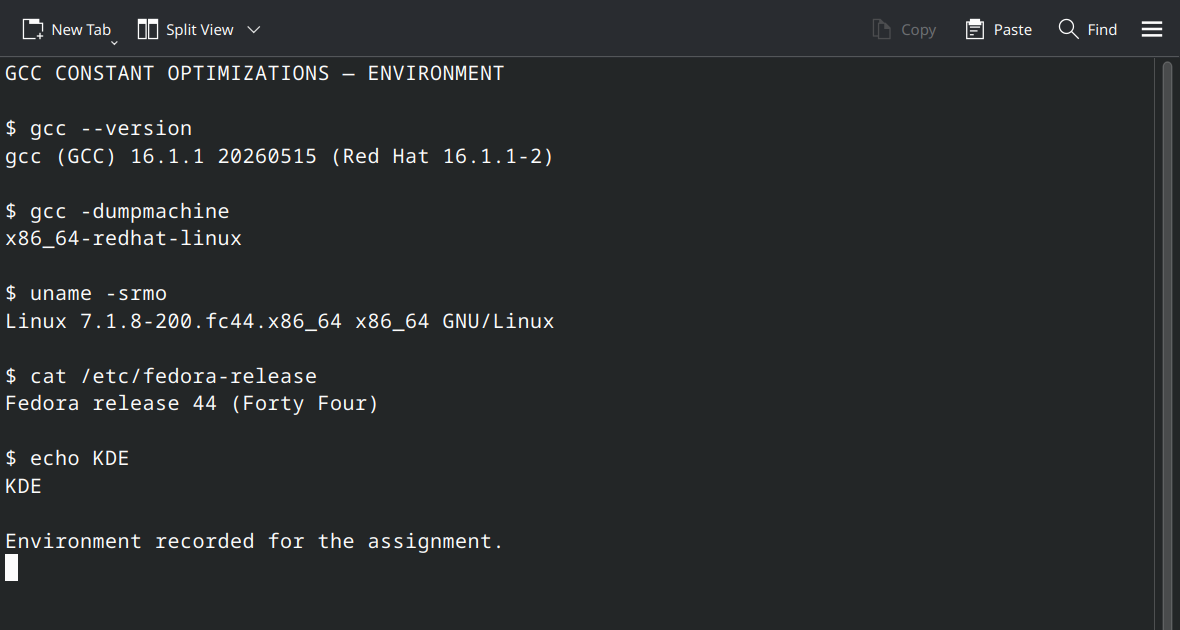
\includegraphics[width=\textwidth]{images/environment.png}
  \caption{GCC version, target, kernel, architecture, and Linux distribution.}
  \label{fig:environment}
\end{figure}

\clearpage

The same command pattern was applied to all three source files, changing the
optimization level and output name as appropriate:

\begin{lstlisting}[numbers=none]
gcc -std=c17 -S -O0 -masm=intel src/folding.c -o asm/folding_O0.s
gcc -std=c17 -S -O1 -masm=intel src/folding.c -o asm/folding_O1.s
gcc -std=c17 -S -O2 -masm=intel src/folding.c -o asm/folding_O2.s
\end{lstlisting}

Before analysis, every source was also checked with the following warning and
syntax options; the checks completed without warnings.

\begin{lstlisting}[numbers=none]
-Wall -Wextra -Wpedantic -fsyntax-only
\end{lstlisting}

\subsection{Meaning of the compiler options}

\begin{description}
  \item[\code{-S}] Compile and stop after emitting assembly rather than
    assembling or linking an executable.
  \item[\code{-O0}] Use GCC's unoptimized baseline. This disables the normal
    optimization pipeline as much as this level specifies, but it does not
    promise a literal, one-instruction-for-each-source-operation translation.
  \item[\code{-O1}] Enable a basic collection of optimizations, including
    transformations that can remove simple temporary values.
  \item[\code{-O2}] Enable additional generally useful optimizations without
    selecting the more aggressive \code{-O3} class.
  \item[\code{-masm=intel}] Request Intel notation in the assembly text. It is
    a presentation choice and does not itself enable optimization.
  \item[\code{-std=c17}] Fix the source-language dialect so that all experiments
    are parsed using the same ISO C rules.
\end{description}

The \code{-O0} qualification is important. A compiler may still evaluate a
literal constant expression during parsing or lowering, or perform other
required and inexpensive simplifications, even when optional optimization
passes are disabled. Therefore the evidence below describes what GCC actually
emitted rather than assuming that \code{-O0} means ``no simplification of any
kind.''

\clearpage
\section{Answer to Part (a): Constant Folding}

Here the arithmetic is written entirely with integer literals, so GCC does not
need to trace any variable values.

\lstinputlisting[language=C,caption={Constant-folding experiment.},label={lst:folding-c}]{src/folding.c}

Even at \code{-O0}, GCC has already evaluated \code{3 * 4 + 2}. The
unoptimized function returns the literal result 14:

\begin{lstlisting}[numbers=none,caption={Relevant \code{-O0} assembly for folding.}]
push    rbp
mov     rbp, rsp
mov     eax, 14
pop     rbp
ret
\end{lstlisting}

With \code{-O1} and \code{-O2}, GCC also removes the frame setup. What remains
is the minimal sequence needed to return the result:

\begin{lstlisting}[numbers=none,caption={Relevant \code{-O1} and \code{-O2} assembly.}]
mov     eax, 14
ret
\end{lstlisting}

\answerline{Yes. GCC 16.1.1 folds this expression at every tested optimization
level, including \code{-O0}. No multiplication or addition remains to be done
at run time.}

\begin{figure}[H]
  \centering
  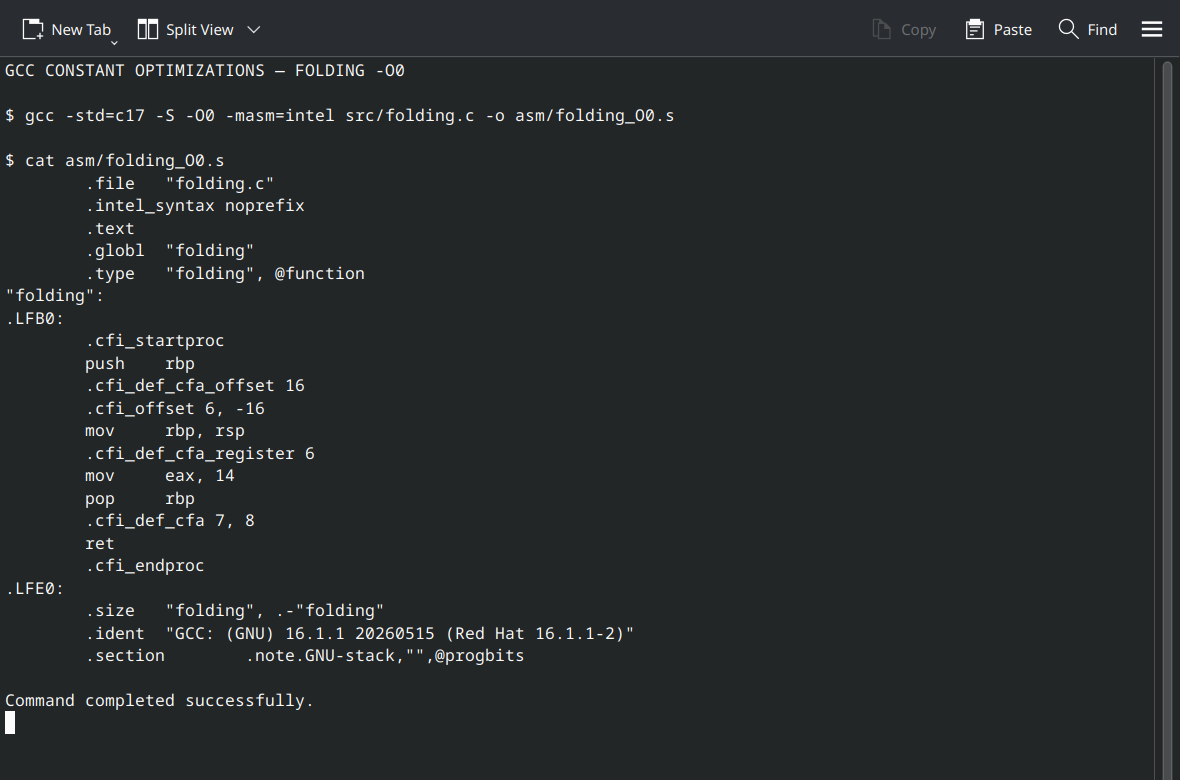
\includegraphics[width=\textwidth]{images/folding_O0.png}
  \caption{Compilation and emitted assembly for folding at \code{-O0}.}
  \label{fig:folding-o0}
\end{figure}

\begin{figure}[H]
  \centering
  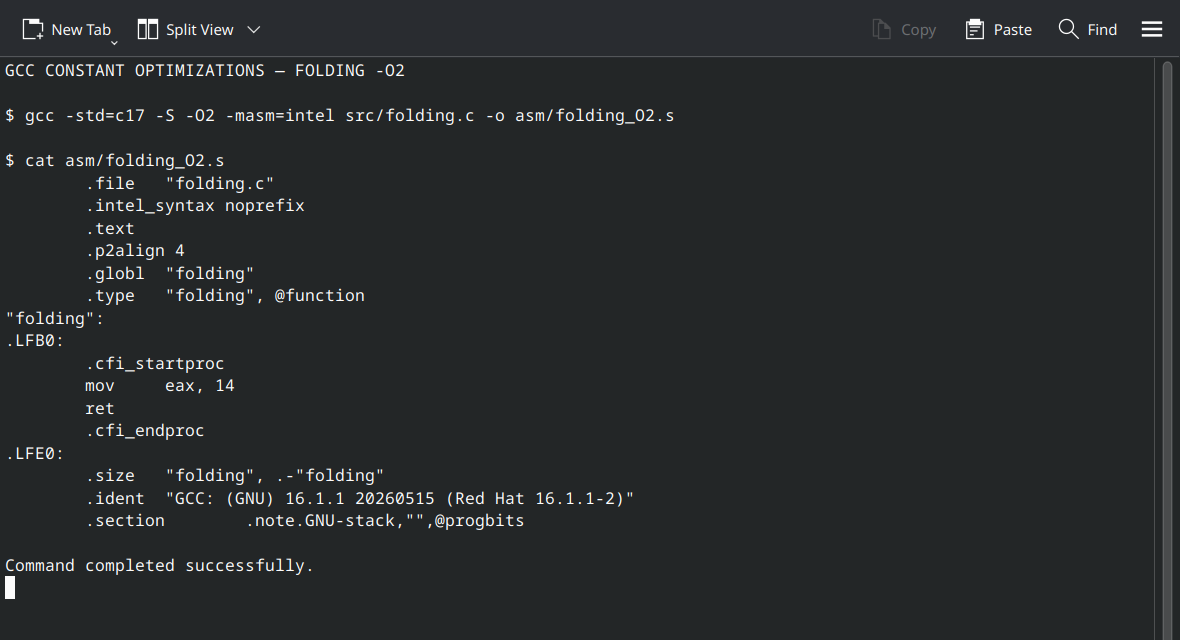
\includegraphics[width=\textwidth]{images/folding_O2.png}
  \caption{Compilation and emitted assembly for folding at \code{-O2}.}
  \label{fig:folding-o2}
\end{figure}

\clearpage
\section{Answer to Part (b): Constant Propagation}

This version places 4 in \code{x}, uses \code{x} to compute \code{y}, and then
returns \code{y}. Before simplifying the result, GCC must follow the value
through those named variables.

\lstinputlisting[language=C,caption={Ordinary-variable propagation experiment.},label={lst:propagation-c}]{src/propagation.c}

At \code{-O0}, GCC keeps that source-level sequence visible. It writes
\code{x} to the stack, reads it back, adds 2, stores \code{y}, and loads
\code{y} again for the return:

\begin{lstlisting}[numbers=none,caption={Relevant \code{-O0} propagation assembly.}]
mov     DWORD PTR [rbp-4], 4
mov     eax, DWORD PTR [rbp-4]
add     eax, 2
mov     DWORD PTR [rbp-8], eax
mov     eax, DWORD PTR [rbp-8]
\end{lstlisting}

Once optimization is enabled, GCC proves which value reaches the return. Both
\code{-O1} and \code{-O2} combine propagation with folding:

\begin{lstlisting}[numbers=none,caption={Relevant \code{-O1} and \code{-O2} propagation assembly.}]
mov     eax, 6
ret
\end{lstlisting}

\answerline{Yes, when optimization is enabled. At \code{-O1} and \code{-O2},
GCC propagates 4 through \code{x}, folds \code{4 + 2}, and returns 6 directly.
At \code{-O0}, it leaves the variable-based operations in place.}

\clearpage

\begin{figure}[H]
  \centering
  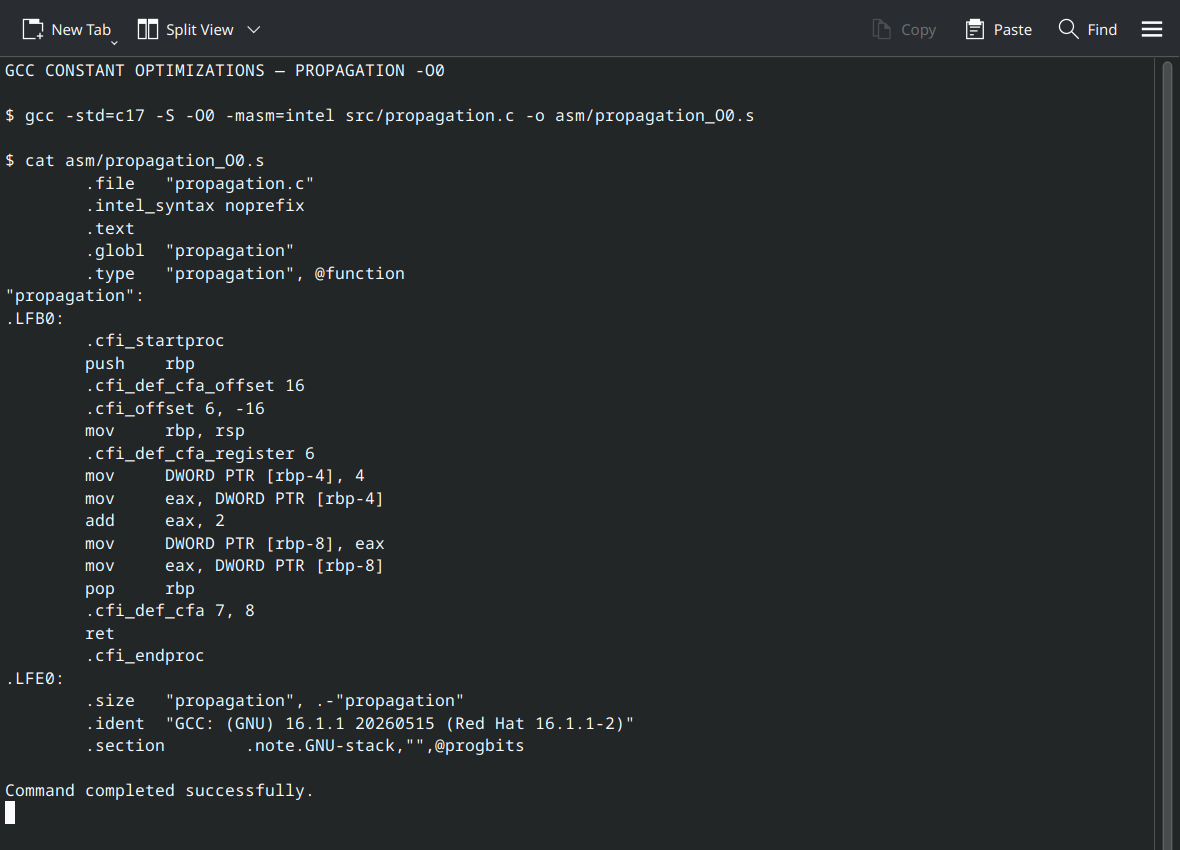
\includegraphics[width=0.92\textwidth]{images/propagation_O0.png}
  \caption{Compilation and emitted assembly for ordinary propagation at \code{-O0}.}
  \label{fig:propagation-o0}
\end{figure}

\begin{figure}[H]
  \centering
  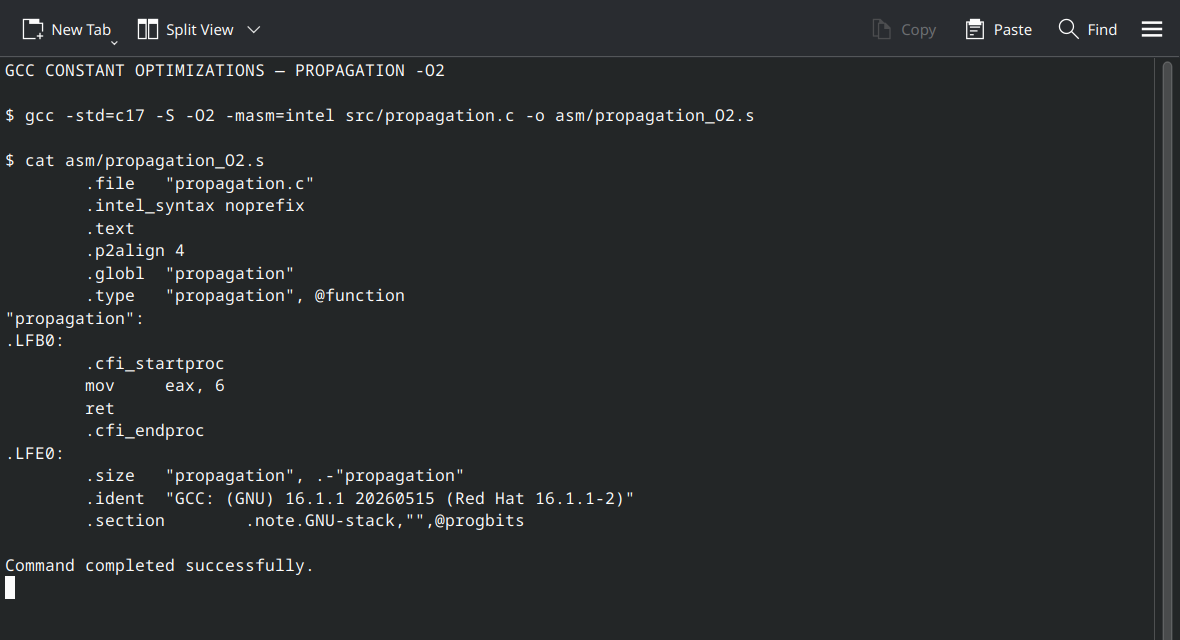
\includegraphics[width=0.92\textwidth]{images/propagation_O2.png}
  \caption{Compilation and emitted assembly for ordinary propagation at \code{-O2}.}
  \label{fig:propagation-o2}
\end{figure}

\clearpage
\section{Answer to Part (c): Why Propagation Is Harder}

Folding starts with constants that are already visible in an expression.
Propagation has an extra job: before substituting a value, the compiler must
prove that the variable still holds it at that exact use. The proof may have to
cross assignments, branches, and other code.

\begin{enumerate}
  \item \textbf{Reassignment.} A variable can begin with a constant and receive
    a different value later. The compiler has to determine which assignment
    reaches each use.
  \item \textbf{Branches and control-flow joins.} Different paths may assign
    different values. After the paths merge, a value is constant only if every
    feasible incoming path agrees.
  \item \textbf{Loops.} An assignment inside a loop can affect the next
    iteration. The compiler may need to analyze the loop repeatedly before it
    reaches a stable conclusion.
  \item \textbf{Pointers and aliasing.} A pointer write may change a variable
    even when the variable's name does not appear in that statement. If GCC
    cannot rule out the alias, it cannot safely keep treating the value as
    constant.
  \item \textbf{Function calls and side effects.} A call may change memory,
    globals, or objects reached through pointers. When GCC lacks enough
    information about the called function, it must assume that such changes are
    possible.
  \item \textbf{Global or external state.} Other functions or separately
    compiled code may change externally visible objects. GCC therefore cannot
    generally treat their values as fixed compile-time constants.
\end{enumerate}

That is why folding is usually local, while propagation is a data-flow problem.
The compiler tracks definitions through the program and stops treating a value
as constant as soon as the proof no longer holds.

\clearpage
\section{Answer to Part (d): Named \code{const} Object}

Only one source-level detail changes in the third program: \code{x} is declared
as a \code{const int}.

\lstinputlisting[language=C,caption={Propagation experiment with a named \code{const} object.},label={lst:const-c}]{src/const_propagation.c}

I compared the raw assembly files with \code{diff -u} at all three levels.
Table~\ref{tab:const-comparison} summarizes what GCC produced.

\begin{table}[H]
  \centering
  \caption{Ordinary versus \code{const} propagation.}
  \label{tab:const-comparison}
  \begin{tabular}{@{}p{0.13\textwidth}p{0.36\textwidth}p{0.39\textwidth}@{}}
    \toprule
    Level & Ordinary variable & Named \code{const} object \\
    \midrule
    \code{-O0} & Store 4, load it, add 2, store and reload the result. & Same executable instruction sequence. \\
    \code{-O1} & \code{mov eax, 6}; \code{ret} & Same executable instruction sequence. \\
    \code{-O2} & \code{mov eax, 6}; \code{ret} & Same executable instruction sequence. \\
    \bottomrule
  \end{tabular}
\end{table}

The textual diffs still report harmless changes in the \code{.file},
\code{.globl}, \code{.type}, function label, and \code{.size} directives. They
use \code{propagation} in one file and \code{const\_propagation} in the other.
These records identify different source files and functions. They do not change
the computation in the instruction body.

\begin{lstlisting}[numbers=none,caption={Instruction body shared by both variants at \code{-O2}.}]
mov     eax, 6
ret
\end{lstlisting}

In C, \code{const int x = 4;} declares \code{x} as an object of const-qualified
type. It therefore is not modifiable through a const-qualified lvalue. The
object may still occupy storage and have an address. A macro works differently:
\code{\#define X 4} tells the preprocessor to replace the token \code{X} with
\code{4} before the compiler analyzes the C program. A named \code{const}
object is not textual substitution.

\answerline{Yes. In this small program, GCC treats the ordinary and
\code{const} versions the same at every tested level. Both retain the variable
operations at \code{-O0}; both propagate and fold the value to a direct return
of 6 at \code{-O1} and \code{-O2}.}

\clearpage

\begin{figure}[H]
  \centering
  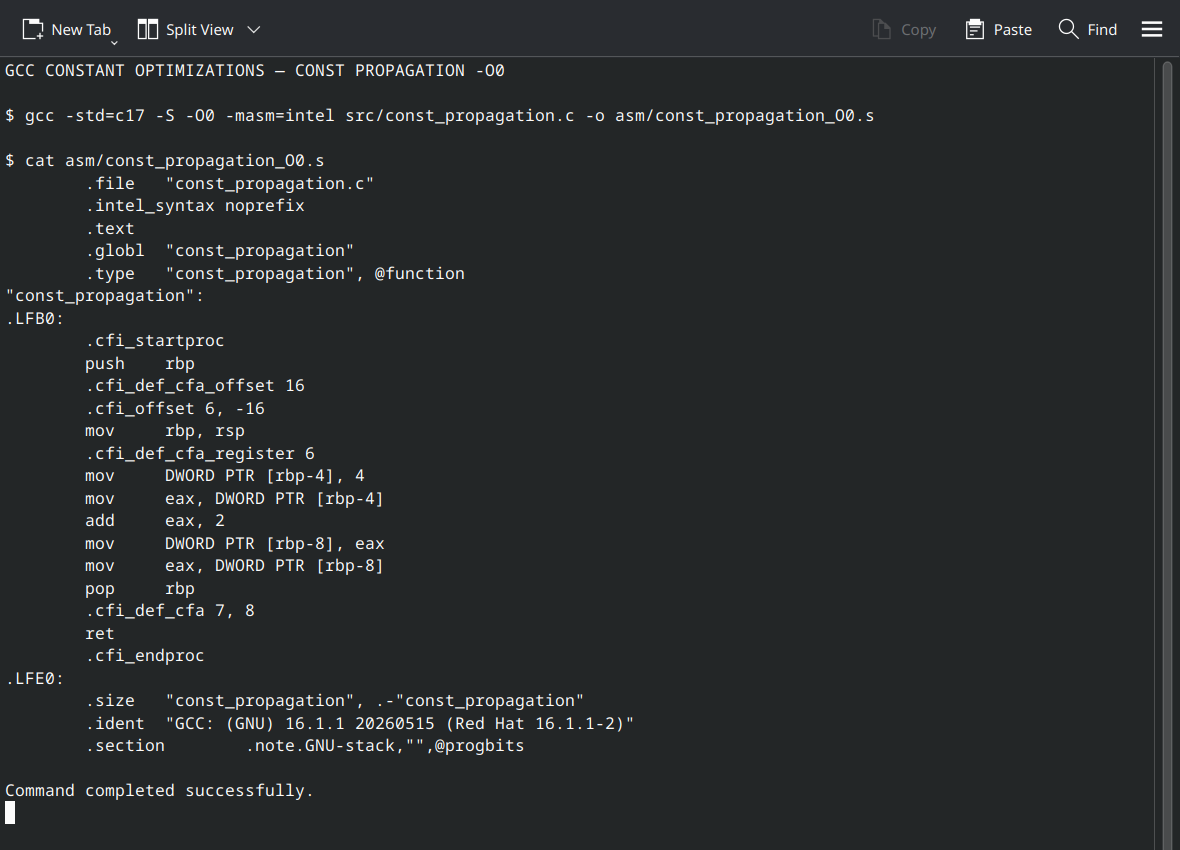
\includegraphics[width=0.92\textwidth]{images/const_propagation_O0.png}
  \caption{Compilation and emitted assembly for named-\code{const} propagation at \code{-O0}.}
  \label{fig:const-o0}
\end{figure}

\begin{figure}[H]
  \centering
  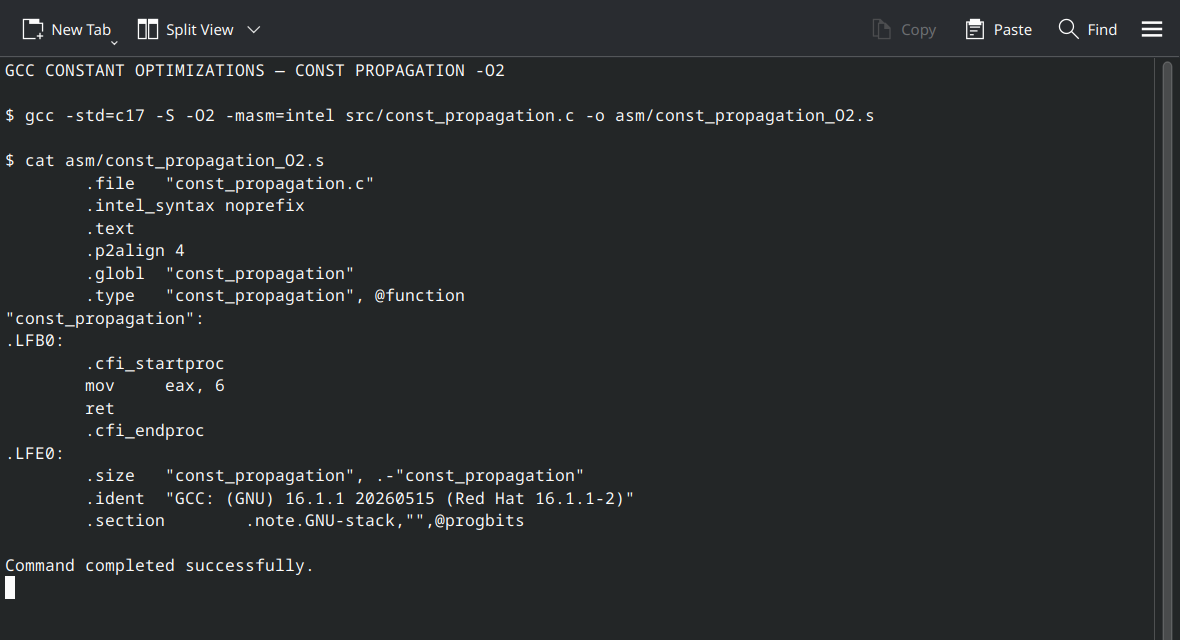
\includegraphics[width=0.92\textwidth]{images/const_propagation_O2.png}
  \caption{Compilation and emitted assembly for named-\code{const} propagation at \code{-O2}.}
  \label{fig:const-o2}
\end{figure}

\clearpage
\section{Conclusion}

The experiments separate two related compiler tasks. GCC folded the purely
literal expression \code{3 * 4 + 2} into 14 even at \code{-O0}. When the value
flowed through variables, \code{-O0} retained the stores, loads, and addition,
whereas \code{-O1} and \code{-O2} propagated the known value and returned 6
directly. Declaring the source variable \code{const} did not alter the
instruction sequence for this program, although the declaration conveys a
source-language restriction that is fundamentally different from a macro.

These are observations for the recorded GCC 16.1.1, x86-64 Fedora environment;
other compiler versions and targets may choose different instruction sequences
while preserving the same C semantics.

\end{document}
